\chapter{CRONOGRAMA}
\label{chap:cronograma}

O cronograma do projeto é apresentado logo abaixo. As tarefas estão separadas em meses, por conta disso, elas possuem um \textit{X} nos meses em que serão trabalhadas. Em verde são as tarefas ou parte delas que já foram concluídas. Já em amarelo, está as tarefas que estão em andamento. Em vermelho, são as que ainda não foram iniciadas.

\begin{figure}[H]
    \centering
    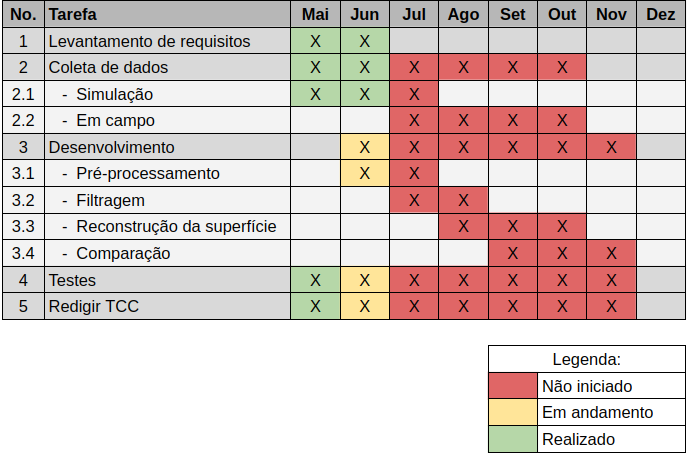
\includegraphics[scale=0.8]{dados/figuras/cronograma.png}
\end{figure}